\subsection{Instance-based learning}
Basic key idea: just store all training examples
\begin{outline}
    \1 When seeing a new instance:
        \2 Find the most similar cases in the database
        \2 make a prediction based on those instance
    \1 Architypical method: k-nearest-neighbors (k-NN)
        \2 use most frequent class/ mean target among the k nearest neighbors as your prediction
        \2 k is chosen by the user (hyperparameter)
    \1 Similarity
        \2 how close to others, often Euclidean distance for numerical inputs
    \1 Voronoi diagrams
        \2 indicate area where prediction is influenced by same set of examples
        \2 for 1-NN: cell borders are right in the middle between any two data points
        \2 This is called a Voronoi diagram - kNN
    \1 Decision surface
        \2 Decision surface separate regions with different predictions
    \1 Voronoi diagram for k > 1
        \2 To construct diagram for k-NN with k > 1
             \3 Start from diagram for k-1
             \3 for each cell:
                \4 temporarily forget about k-1 nearest neighbors
                \4 split cell according to k'th nearest neighbors
            \3 Merge adjacent cells with same k nearest neighbors
    \1 pros vs. cons
        \2 \textbf{pros}
            \3 "Learning" is very fast - just storing the data
            \3 all detials of the data are kept
        \2 \textbf{cons}
            \3 can be slow at prediction time
            \3 difficulties in high-dimensional spaces
            \3 relies on having a good similarity measure (Euclidean distance - numerical)
            \3 not robust to noise
    \1 for k-NN, large K -> more robust to overfitting? but it is more robust to noise
    \1 difficulties with high-dimensional space - curse of dimensionality - data are distribtued very sparsely in high-D
    \1 Improvement: Different scales
        \2 When dimensions have very differnet scales, Euclidean distance may not work well
            \3 Solution: normalization - normalize all dimensions to comparable scale
            \3 Give irrelevant dimensions a smalelr weight in the Euclidean distance, so they have less influence
            \3 using a closed formula: $w_{i} = 1 - \frac{1}{n} \sum_{k=1}^{c} \sum_{j=1}^{n_{k}} |\bar{x}_{ki} - x_{kji}|$
            \3 with $c$=\#clusters, $n_{k}$=\#elements in cluster k, $x_{ki}$=mean $x_{i}$ in cluster k, $x_{kji}$=$x_{i}$ for j\'th element in cluster k
    \1 Improvenment: distance-werights k-NN
        \2 Why 3-NN, but why not 4-NN
            \3 Solution: no cut-off at k, but have weights gradually decrease with distance
            \3 careful: influence must decrease fast with distance, otherwise faraway cases will dominate the voting (otherwise noise)
    \1 Improvement: locally weighted regression
        \2 for better fitting
            \3 Solution: fit a simple local model
            \3 a linear regression can be okay
    \1 Prototypes
        \2 A prototype is a representattive for a group of instances
        \2 can be an average for elements in a cluster
        \2 note: need to define similarity between instance \& prototype
    \1 Efficient prediction
        \2 Solution: indexing the data helps
\end{outline}

\begin{outline}
    \1 Lazy learners vs. eager learners
        \2 k-NN is called lazy learner
            \3 do not build a model during training, merely store data
            \3 start doing the hard work when asked a question
        \2 eager learners
            \3 generalize before knowing the question
            \3 try to build a global model that will owrk under all circumstances
        \2 lazy learners can use simpler local models - sometime very accurate
            \3 compare: locally weighted linear regression (k-NN) vs. global linear regression
            \3 compare: learn one rule that covers the query instance vs. learn a global rule set
\end{outline}

\subsection{Clustering}
\begin{outline}
    \1 Overview
        \2 Find structure/pattern in the data, in the form of groups of instances that are highly similar to each other
        \2 It is unsupervised machine learning (no labeled samples)
    \1 Find groups (clusters) of instances so that
        \2 instances in the same group are similar
        \2 instances in the difference group are different 
    \1 Definition of clustering
        \2 flat clustering
            \3 returns a partition of the data
        \2 hierarchical clustering
            \3 returns a hierarchy of clusters
    \1 Other definition of clustering
        \2 extensional clustering
            \3 clusters are defined without any description language
        \2 conceptual clustering
            \3 clusters are defiend using a conceptual description language
\end{outline}

\begin{figure}[htbp]
    \centering
    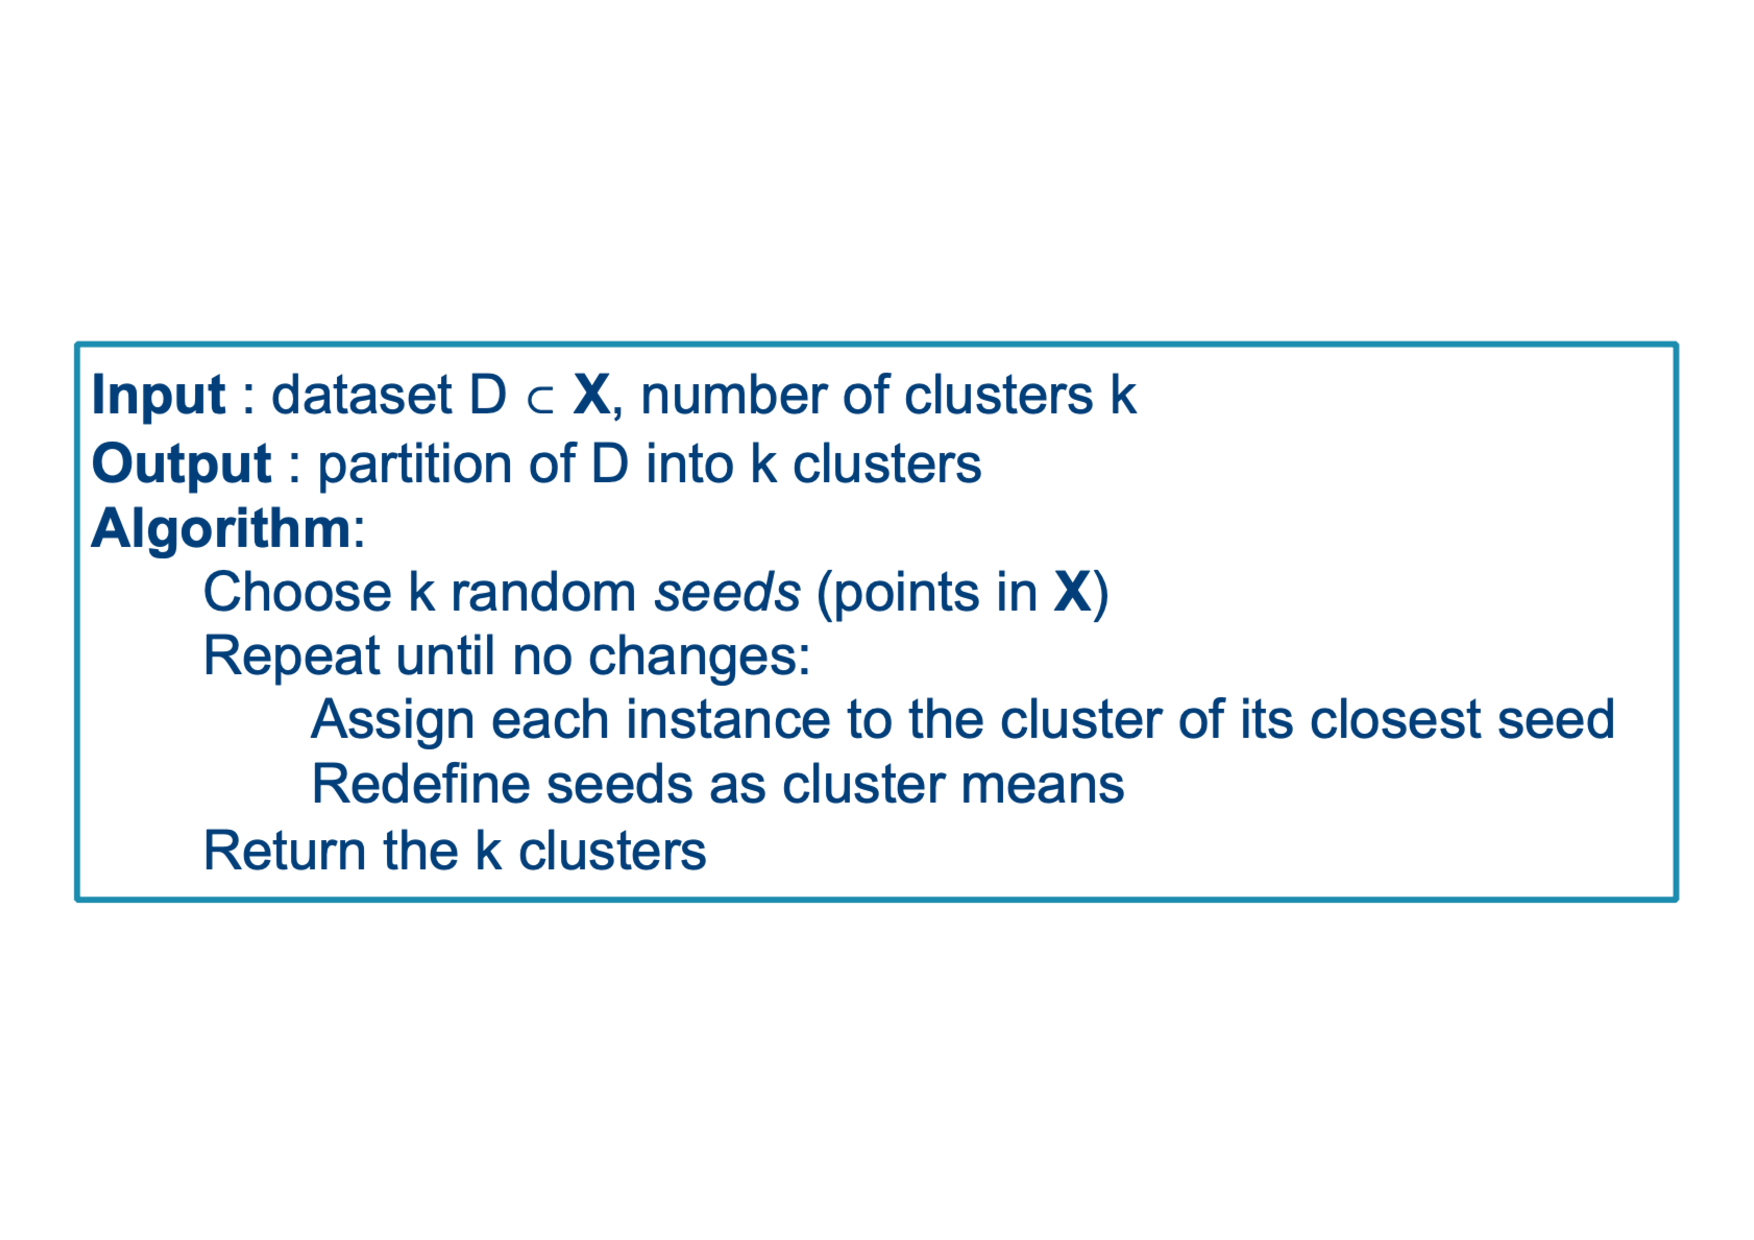
\includegraphics[height=4cm]{../figs/kmean_algorithm.pdf}
    \caption{Algorithm for "Algorithm for flat, extensional clustering: K-means"}
    \label{fig:kmeans_algorithm}
\end{figure}

\begin{outline}
    \1 FLat, extensional clustering
        \2 task: given a set of unlabeled data, find groups of highly similar instances
        \2 some constraints may additionally be given
        \2 procedure: reassign points, recompute seeds, reassign points ..., when no points are re-assigned to another cluster, stop.
    \1 Hierarchical, extensional clustering
        \2 top-down ("divisive") methods
            \3 start with 1 cluster (whole data set)
            \3 divide it into subsets
            \3 subdivide subsets further
        \2 bottom-up ("agglomerative") methods
            \3 start with singleton clusters
            \3 join closest clusters together
            \3 repeat until 1 cluster
    \1 Bottom-up methods
        \2 How does it generalize to distance between clusters? - based on examples
            \3 Single linkage: distance between clusters = distance between each closest point in their cluster
            \3 Complete linkage: distance between clusters = distance between each furthest poin in their clusters
            \3 Average linkage: distance between clusters = distance between average of clusters 
    \1 Conceptual clustering
        \2 Cluster + find a conceptual description of each cluster (in some given description language L)
        \2 Clearly, the clusters are not defined using distance alone! Context is improtant!
    \1 Examples: Cobweb
        \2 Predictability: given cluster, how well can you predict attribute values
        \2 Predictiveness: given attribute values, how well can you predict cluster
        \2 Cobweb is to maximize a combination of both
    \1 Decision tree learning, viewed as clustering
        \2 A decision tree defines a conceptual, hierarchical clustering of the data
            \3 each node = subset of the data
            \3 conceptual description of these data = conjunction of test outcomes from root to node
    \1 Clustering trees
        \2 for regression (original), heuristic minimize average variance of Y within subsets
            \3 $Var(S) = \sum_{(x,y) \in S} \frac{(y - \bar{y})^{2}}{|S|-1|}$ 
            \3 with $\bar{y} = \sum_{(x,y) \in S} \frac{y}{|S|}$
        \2 for clustering (unsupervised clustering tree), given some distance metric d that indicates dissimilarity, we can minimize the average variance of X wihtin subsets
            \3 $Var(S) = \sum_{x \in S} \frac{d(x,\bar{x})^{2}}{|S|-1}$
            \3 with $\bar{x} = \sum_{x \in S} \frac{x}{|S|}$
    \1 Predictive clustering
        \2 overview: it looks like from value -> cluster and from cluster -> value
        \2 Predictive clustering builds a model consisting of 
            \3 a set of clusters
            \3 a function c assigning instances to clusters
            \3 a function p assigning a target value to the instance, given the cluster
        \2 the overall predictive function is then $f(x) = p(c(x),x)$
        \2 the accuracy of f will depend on that of c and p.
            \3 an accurate c requires good predictiveness (from value to cluster)
            \3 an accurate p requires good Predictability (from cluster to value)
\end{outline}

\begin{figure}[htbp]
    \centering
    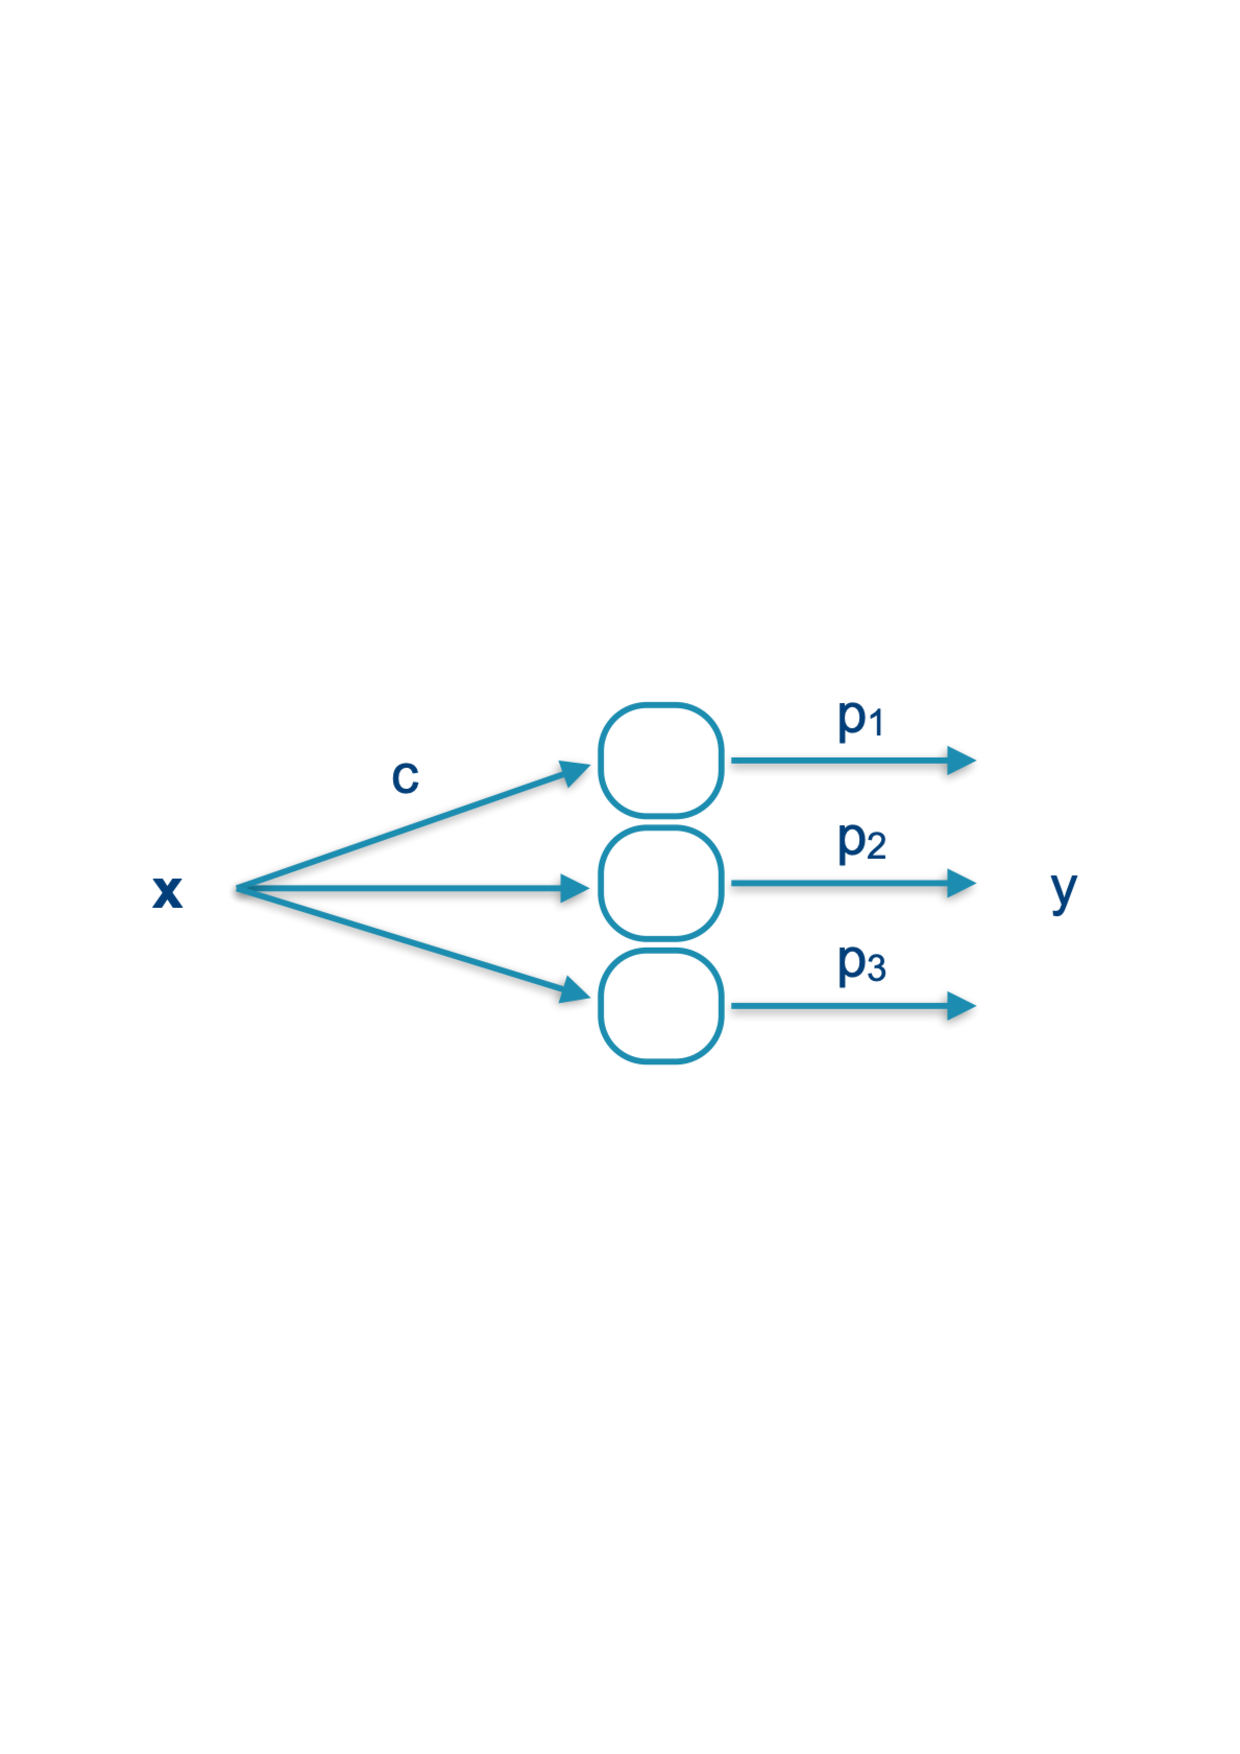
\includegraphics[height=4cm]{../figs/predictive_cluster_scheme.pdf}
    \caption{Algorithm for "Scheme of Predicttive Cluster"}
    \label{fig:scheme_predictive_cluster}
\end{figure}

\begin{outline}
    \1 Similarity measures
        \2 Similarity is often represented using a distance metric
            \3 small distance = high similarity, e.g., euclidean distance, manhattan distance, hamming distance, ...
            \3 $d_{Eucl}(x,x^{\prime}) = \sqrt{\sum_{i} (x_{i}-x_{i}^{\prime})^{2}}$
            \3 $d_{Manh}(x,x^{\prime}) = \sum_{i} |x_{i} - x_{i}^{\prime}|$
        \2 Not all similarity measures can be expressed in that way!
            \3 Distance metric fulfills symmetry and triangle inequality
            \3 Some similarity measures cannot be mapped to such a distance measures
    \1 Learning the similarity measure
        \2 Clustering relies strongly on defining an appropriate similarity measure
        \2 However, this may be very difficult sometime
            \3 Solution: semi-supervised clustering
            \3 Computer learns the similarity from examples of pairs of instances that should be in the same/ in differrent clusters, "must-link" and "cannot-link" constraints
            \3 then start the unlabeled data, (semi-supervised clustering: a few labeled data, many unlabeled data)
    \1 Learning preferred clusterings
        \2 Different clustering algorithms have different biases
            \3 k-means: spherical clusters
            \3 density-based: can return concave clusters
            \3 some methods can even return disconnected cluster
    \1 example of interactive clustering: the COBRAS method
        \2 using an intermediate level of super-instances
            \3 clustering = set of clusters
            \3 cluster = set of super-instances
            \3 super-instance = set of clusters
    \1 Evaluating clusterings
        \2 How can we assess whether a clustering is good or bad?
        \2 explicit objective: minimize intra-cluster variance
        \2 internal criteria: inherent to the clustering
        \2 external criteria: compare to a reference clustering
            \3 rand (random) index
            \3 adjusted rand (random) index (ARI)
\end{outline}
\pagebreak
